% Yeban User Guide — Chapter 7: Mixer Overview (English)
% T-DOC-001 chapter-by-chapter delivery, written ahead of the CH07 task.
% Sources: app.slint mixer/send/control-room callbacks and menus,
% docs/manual/05-mixer-effects.md, cli.rs SHORTCUTS.

\chapter{Mixer Overview}
\label{ch:mixer-overview}

\begin{quote}
八音克谐，无相夺伦。
\end{quote}

Source: Book of Documents, “Canon of Shun” (《尚书·舜典》). Translation: “Let the eight sounds harmonize, without one usurping another’s place.”

Mixing lets tracks coexist without masking each other; the whole matters more than any single sound.

This chapter follows a signal from a track to the master bus: what a channel strip
holds, in what order inserts take effect, how sends and buses are wired, and where to
watch master monitoring and loudness. Individual effect parameters are out of scope.

\section{Channel Strips and Insert Chains}

\subsection{Open the mixer console}

Press X, or switch to the mixer console in the bottom dock (F8 is also a direct key).
Each track has one channel strip: its volume fader at the top, pan, mute/solo, and the
entry to that track's device chain. All tracks eventually sum into the master bus.

Mix $\to$ Reset Master Fader to 0dB zeroes the master fader in one step — that is a
shortcut for the master bus and does not touch any track fader. The left inspector (I)
shows the same channel-strip details for the selected track; it is the same state as
the mixer, so changes in either place agree.

\screenshot{ch07-mixer-console}{The mixer console in full, labelling channel strips, faders, mute/solo and the master bus}

\subsection{Device chain: instruments first, effects after}

Each track has a device chain: instruments first, effects after, and the order is the
signal-flow order. The bottom Device Rack tab (F9) lets you add/remove devices and
toggle bypass; bypass is per-device and is not the same as deleting a device.

The Track menu can insert three common devices directly into the current track:
Parametric EQ (frequency shaping), Spatial Reverb (a sense of space) and Dynamic
Compressor (taming dynamics, bringing a sound forward). Device parameters can be
automated: expand an automation lane in the arrangement area (A) and parameter-over-
time changes are recorded with the project and applied on export (Chapter 6).

\begin{figure}[htbp]
\centering
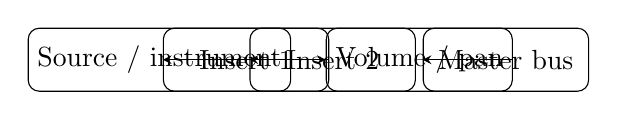
\begin{tikzpicture}[node distance=1.1cm, >=stealth,
    box/.style={draw, rounded corners, align=center, minimum width=2.1cm, minimum height=0.8cm}]
  \node[box] (a) {Source / instrument};
  \node[box, right of=a] (b) {Insert 1};
  \node[box, right of=b] (c) {Insert 2};
  \node[box, right of=c] (d) {Volume / pan};
  \node[box, right of=d] (e) {Master bus};
  \draw[->] (a)--(b); \draw[->] (b)--(c); \draw[->] (c)--(d); \draw[->] (d)--(e);
\end{tikzpicture}
\caption{Signal order: instrument $\to$ inserts (chain order) $\to$ fader/pan $\to$ master bus}
\label{fig:ch07-signal-flow}
\end{figure}

\section{Sends, Buses and the Control Room}

\subsection{Sends and aux buses}

A send routes a copy of one path's signal to another path; an aux bus track (Track
$\to$ New Aux Bus Track) receives those sends for summing or group processing. Sends
can be created and removed from the interface and their gain adjusted; when creation
conditions are not met, the interface states the reason rather than failing silently.

\screenshot{ch07-sends}{The sends area on a channel strip showing destination buses, gain and create/remove entries}

\subsection{Control Room}

Mix $\to$ Show/Hide Control Room (shortcut F4) opens a separate master-monitoring
area: master-bus level and loudness readings, letting you set overall volume without
touching any track fader. It is distinct from the bottom mixer console: the former
governs "what you hear overall", the latter "how each track is balanced".

\screenshot{ch07-control-room}{The Control Room panel showing master-bus level and loudness readings}

\section{Division of Labour with the Mixing Manual}

This chapter is an overview only: where to find controls, roughly how a signal flows,
and how sends and buses are wired. Each effect's parameters, ranges and typical uses
belong to the separate Mixing and Effects manual, which documents them against real
parameter names in the code. The two agree in approach: this chapter says "where",
that volume says "how to adjust".

\section{Help Topic Mapping}

\begin{table}[htbp]
\centering
\caption{Sections of this chapter $\to$ in-app help anchors}
\label{tab:ch07-help}
\begin{tabular}{ll}
\hline
Section & Help topic \\
\hline
Open mixer / channel strip & \texttt{mixer-channel-strip} \\
Insert chain order & \texttt{mixer-insert-chain} \\
Sends and aux buses & \texttt{mixer-sends-buses} \\
Control Room & \texttt{mixer-control-room} \\
Division with the mixing manual & \texttt{mixer-manual-division} \\
\hline
\end{tabular}
\end{table}

\paragraph{What you will be able to do} Find channel strips and the device chain, explain a signal's order, create an aux bus with a send, and know where master monitoring lives.

\paragraph{Hands-on exercise} Press X to open the mixer, insert Parametric EQ on a track and bypass/restore it once from the device rack; create an aux bus track, add a send from the original track and lower its gain; press F4 for the Control Room and read the master-bus level; finally reset the master fader to 0dB and confirm the track faders did not move.
